% RMS wrote:
%The text does not mention GNU anywhere.  This paper is an opportunity
%to make people aware of GNU, but the current text fails to use the
%opportunity.
%
%It should say that Taler is a GNU package.
%
%I suggest using the term "GNU Taler" in the title, once in the
%abstract, and the first time the name is mentioned in the body text.
%In the body text, it can have a footnote with more information
%including a reference to http://gnu.org/gnu/the-gnu-project.html.
%
%At the top of page 3, where it says "a free software implementation",
%it should add "(free as in freedom)", with a reference to
%http://gnu.org/philosophy/free-sw.html and
%http://gnu.org/philosophy/free-software-even-more-important.html.
%
%Would you please include these things in every article or posting?
%
% CG adds:
% We SHOULD do this for the FINAL paper, not for the anon submission.

% Relate to:
% http://fc14.ifca.ai/papers/fc14_submission_124.pdf

% Terminology:
% - SEPA-transfer -- avoid 'SEPA transaction' as we use
%       'transaction' already when we talk about taxable
%        transfers of Taler coins and database 'transactions'.
% - wallet = coins at customer
% - reserve = currency entrusted to exchange waiting for withdrawal
% - deposit = SEPA to exchange
% - withdrawal = exchange to customer
% - spending = customer to merchant
% - redeeming = merchant to exchange (and then exchange SEPA to merchant)
% - refreshing = customer-exchange-customer
% - dirty coin = coin with exposed public key
% - fresh coin = coin that was refreshed or is new
% - denomination key = exchange's online key used to (blindly) sign coin
% - reserve key = key used to authorize withdrawals from a reserve
% - message signing key = exchange's online key to sign exchange messages
% - exchange master key = exchange's key used to sign other exchange keys
% - owner = entity that knows coin private key
% - transaction = coin ownership transfer that should be taxed
% - sharing = coin copying that should not be taxed

% FIXME: As a general comment, I think we're mixing the crypto stuff and the systems
%        stuff too much.  It might be more appropriate to have to systems stuff in a separate
%        section, and the "pure" crypto stuff for the crypto people?


\documentclass[sigconf, authordraft]{acmart}

\usepackage{booktabs} % For formal tables
\usepackage{tikz}
\usetikzlibrary{shapes,arrows}
\usetikzlibrary{positioning}
\usetikzlibrary{calc}
\usepackage{eurosym}


% Copyright
%\setcopyright{none}
%\setcopyright{acmcopyright}
%\setcopyright{acmlicensed}
\setcopyright{rightsretained}
%\setcopyright{usgov}
%\setcopyright{usgovmixed}
%\setcopyright{cagov}
%\setcopyright{cagovmixed}


% DOI
\acmDOI{10.475/123_4}

% ISBN
\acmISBN{123-4567-24-567/08/06}

%Conference
\acmConference[WOODSTOCK'97]{ACM Woodstock conference}{July 1997}{El
  Paso, Texas USA}
\acmYear{1997}
\copyrightyear{2016}

\acmPrice{15.00}

\acmSubmissionID{123-A12-B3}

\begin{document}
\title{Refreshing Coins for Giving Change and Refunds \\ in Chaum-style Anonymous Payment Systems}
\subtitle{Authors' names blinded for review}


%\author{Ben Trovato}
%\authornote{Dr.~Trovato insisted his name be first.}
%\orcid{1234-5678-9012}
%\affiliation{%
%  \institution{Institute for Clarity in Documentation}
%  \streetaddress{P.O. Box 1212}
%  \city{Dublin}
%  \state{Ohio}
%  \postcode{43017-6221}
%}
%\email{trovato@corporation.com}


% The default list of authors is too long for headers}
%\renewcommand{\shortauthors}{B. Trovato et al.}


\begin{abstract}
This paper introduces {\em Taler}, a Chaum-style digital payment system that
enables anonymous payments while ensuring that entities that receive
payments are auditable.  In Taler, customers can
never defraud anyone, merchants can only fail to deliver the
merchandise to the customer, and payment service providers are
audited.
All parties receive cryptographic evidence for all
transactions; still, each party only receives the minimum information
required to execute transactions.  Enforcement of honest behavior is
timely, and is at least as strict as with legacy credit card payment
systems that do not provide for privacy.

The key technical contribution underpinning Taler is a new {\em
  refresh protocol} which allows fractional payments and refunds while
maintaining untraceability of the customer and unlinkability of
transactions.  The refresh protocol combines an
efficient cut-and-choose mechanism with a {\em link} step to ensure
that refreshing is not abused for transactional payments.

We argue that Taler provides a secure digital payment system for modern
liberal societies as it is a flexible, libre and efficient protocol
and adequately balances the state's need for monetary control with the
citizen's needs for private economic activity.
\end{abstract}

%
% The code below should be generated by the tool at
% http://dl.acm.org/ccs.cfm
% Please copy and paste the code instead of the example below.
%
\begin{CCSXML}
<ccs2012>
 <concept>
  <concept_id>10010520.10010553.10010562</concept_id>
  <concept_desc>Computer systems organization~Embedded systems</concept_desc>
  <concept_significance>500</concept_significance>
 </concept>
 <concept>
  <concept_id>10010520.10010575.10010755</concept_id>
  <concept_desc>Computer systems organization~Redundancy</concept_desc>
  <concept_significance>300</concept_significance>
 </concept>
 <concept>
  <concept_id>10010520.10010553.10010554</concept_id>
  <concept_desc>Computer systems organization~Robotics</concept_desc>
  <concept_significance>100</concept_significance>
 </concept>
 <concept>
  <concept_id>10003033.10003083.10003095</concept_id>
  <concept_desc>Networks~Network reliability</concept_desc>
  <concept_significance>100</concept_significance>
 </concept>
</ccs2012>
\end{CCSXML}

\ccsdesc[500]{Computer systems organization~Embedded systems}
\ccsdesc[300]{Computer systems organization~Redundancy}
\ccsdesc{Computer systems organization~Robotics}
\ccsdesc[100]{Networks~Network reliability}


\keywords{ACM proceedings, \LaTeX, text tagging}

\maketitle

\section{Introduction}

The design of payment systems shapes economies and societies.  Strong,
developed nation states have adopted highly transparent payment systems,
such as the MasterCard and VisaCard credit card schemes and computerized
bank transactions such as SWIFT.  These systems enable mass surveillance
by both governments and private companies.  Aspects of this surveillance
sometimes benefit society by providing information about tax evasion or
crimes like extortion.
%
%In particular, bribery and corruption are limited to elites who can
%afford to escape the dragnet.
%
At the other extreme, weaker developing nation states have economic
activity based largely on coins, paper money or even barter.  Here,
the state is often unable to effectively monitor or tax economic
activity, and this limits the ability of the state to shape the
society.
% If we remove the sentence above, this one also needs to go as it
% is the dual...
% As bribery is virtually impossible to detect, corruption is
% widespread and not limited to social elites.
%
%
% SHORTER: Zerocash need not be mentioned so early?
% Zerocash~\cite{zerocash} is an example for translating an
% anarchistic economy into the digital realm.

This paper describes Taler, a simple and practical payment system
which balances accountability and privacy.

The Taler protocol is an improvement over Chaum's original
design~\cite{chaum1983blind} and also follows Chaum's basic
architecture of customer, merchant and exchange
(Figure~\ref{fig:cmm}).  The two designs share the key first step
where the {\em customer} withdraws digital {\em coins} from the {\em
  exchange} with unlinkability provided via blind signatures.  The
coins can then be spent at a {\em merchant} who {\em deposits} them at
the exchange.  Taler uses online detection of double-spending and
provides fair exchange and exculpability via cryptographic proofs.
% Thus merchants are instantly assured that a transaction is valid.

\begin{figure}[h]
\centering
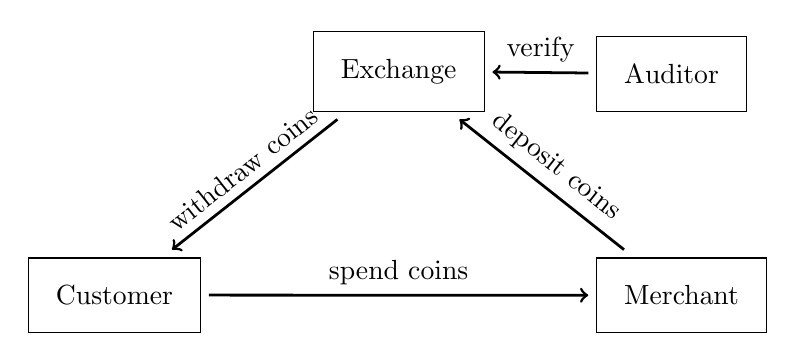
\begin{tikzpicture}
 \tikzstyle{def} = [node distance= 2em and 6.5em, inner sep=1em, outer sep=.3em];
 \node (origin) at (0,0) {};
 \node (exchange) [def,above=of origin,draw]{Exchange};
 \node (customer) [def, draw, below left=of origin] {Customer};
 \node (merchant) [def, draw, below right=of origin] {Merchant};
 \node (auditor) [def, draw, above right=of origin]{Auditor};

 \tikzstyle{C} = [color=black, line width=1pt]

 \draw [<-, C] (customer) -- (exchange) node [midway, above, sloped] (TextNode) {withdraw coins};
 \draw [<-, C] (exchange) -- (merchant) node [midway, above, sloped] (TextNode) {deposit coins};
 \draw [<-, C] (merchant) -- (customer) node [midway, above, sloped] (TextNode) {spend coins};
 \draw [<-, C] (exchange) -- (auditor) node [midway, above, sloped] (TextNode) {verify};

\end{tikzpicture}
\caption{Taler's system model for the payment system is based on Chaum~\cite{chaum1983blind}.}
\label{fig:cmm}
\end{figure}

A key issue for an efficient Chaumian digital payment system is the
need to provide change and existing systems for ``practical
divisible'' electronic cash have transaction costs that are linear in
the amount of value being transacted, sometimes hidden in the double
spending detection logic of the payment service
provider~\cite{martens2015practical}.  The customer should also not be
expected to withdraw exact change, as doing so reduces anonymity due
to the obvious correlation.

% FIXME:  explain the logarithmic claim!  It's only
% true for a certain denomination structure.
% This denomination structure potentially introduces privacy risks
Taler solves the problem of giving change by introducing a new {\em
  refresh protocol} allowing for ``divisible'' transactions with
amortized costs logarithmic in the amount of value being transacted.
Using this protocol, a customer can obtain change or refunds in the
form of fresh coins that other parties cannot link to the original
transaction, the original coin, or each other.  Additionally, the
refresh protocol ensures that the change is owned by the same entity
which owned the original coin.


%\vspace{-0.3cm}

\section{Related Work}
%\vspace{-0.3cm}

%\subsection{Blockchain-based currencies}

% FIXME:  SHORTEN.  This is probably too much information for the audience, they
%         all know this
In recent years, a class of decentralized electronic payment systems,
based on collectively recorded and verified append-only public
ledgers, have gained immense popularity.  The most well-known protocol
in this class is Bitcoin~\cite{nakamoto2008bitcoin}.  The key
contribution of blockchain-based protocols is that they dispense with
the need for a central, trusted authority.  Yet, there are several
major irredeemable problems inherent in their designs:

\begin{itemize}
  \item The computational puzzles solved by Bitcoin nodes with the purpose
    of securing the blockchain consume a considerable amount of energy.
    So Bitcoin is an environmentally irresponsible design.
  \item Bitcoin transactions have pseudonymous recipients, making taxation
    hard to systematically enforce.
  \item Bitcoin introduces a new currency, creating additional
    financial risks from currency fluctuation.
  \item Anyone can start an alternative Bitcoin transaction chain,
    called an AltCoin, and, if successful, reap the benefits of the low
    cost to initially create coins cheaply as the proof-of-work
    difficulty adjusts to the computation power of all
    miners in the network.  As participants are
    de facto investors, AltCoins become a form of Ponzi scheme.
    % As a result, dozens of
    % AltCoins have been created, often without any significant changes to the
    % technology.  A large number of AltCoins creates additional overheads for
    % currency exchange and exacerbates the problems with currency fluctuations.
\end{itemize}

Bitcoin also lacks anonymity, as all Bitcoin transactions are recorded
for eternity, which can enable identification of users.  Anonymous
payment systems based on Bitcoin such as CryptoNote~\cite{cryptonote}
(Monero), Zerocash~\cite{zerocash} (ZCash) and BOLT~\cite{BOLT}
exacerbate the design issues we mention above.  These systems exploit the
blockchain's decentralized nature to escape anti-money laundering
regulation~\cite{molander1998cyberpayments} as they provide anonymous,
disintermediated transactions.

GreenCoinX\footnote{\url{https://www.greencoinx.com/}} is a more
recent AltCoin where the company promises to identify the owner of
each coin via e-mail addresses and phone numbers.  While it is unclear
from their technical description how this identification would be
enforced against a determined adversary, the resulting payment system
would also merely impose a financial panopticon on a Bitcoin-style
money supply and transaction model.

%\subsection{Chaum-style electronic cash}

Chaum~\cite{chaum1983blind} proposed a digital payment system that
would provide some customer anonymity while disclosing the identity of
the merchants.  DigiCash, a commercial implementation of Chaum's
proposal ultimately failed to be widely adopted.  In our assessment,
key reasons for DigiCash's failure include:

\begin{itemize}
 \item The use of patents to protect the technology; a payment system
   should be free software (libre) to have a chance for widespread adoption.
 \item Support for payments to off-line merchants, and thus deferred
   detection of double-spending, requires the exchange to attempt to
   recover funds from delinquent customers via the legal system.
   Any system that fails to be self-enforcing creates a major
   business risk for the exchange and merchants.
%   In 1983, there were merchants without network connectivity, making that
%   feature relevant, but today network connectivity is feasible for most
%   merchants, and saves both the exchange and merchants the business risks
%   associated with deferred fraud detection.
 \item % In addition to the risk of legal disputes wh fraudulent
   % merchants and customers,
   Chaum's published design does not clearly
   limit the financial damage a exchange might suffer from the
   disclosure of its private online signing key.
 \item Chaum did not support fractional payments or refunds without
   weakening customer anonymity.
%, and Brand's
%   extensions for fractional payments broke unlinkability and thus
%   limited anonymity.
% \item Chaum's system was implemented at a time where the US market
%   was still dominated by paper checks and the European market was
%   fragmented into dozens of currencies.  Today, SEPA provides a
%   unified currency and currency transfer method for most of Europe,
%   significantly lowering the barrier to entry into this domain for
%   a larger market.
\end{itemize}

To our knowledge, the only publicly available effort to implement
Chaum's idea is Opencoin~\cite{dent2008extensions}.  However, Opencoin
is neither actively developed nor used, and it is not clear
to what degree the implementation is even complete.  Only a partial
description of the Opencoin protocol is available to date.
% FIXME: ask OpenCoin dev's about this! Then make statement firmer!

% FIXME:  not only by brands.  this formulation sounds like
% we're unaware of the huge body of work in the area that is still growing.
Chaum's original digital cash system~\cite{chaum1983blind} was
extended by Brands~\cite{brands1993efficient} with the ability to {\em
  divide} coins and thus spend certain fractions of a coin using
restrictive blind signatures.  Restrictive blind signatures create
privacy risks: if a transaction is interrupted, then any coins sent
to the merchant become tainted, but may never arrive or be spent.
It becomes tricky to extract the value of the tainted coins without
linking to the aborted transaction and risking deanonymization.

Ian Goldberg's HINDE system allowed the merchant to provide change,
but the mechanism could be abused to hide income from
taxation.\footnote{Description based on personal communication. HINDE
  was never published.}
In~\cite{brands1993efficient}, $k$-show signatures were proposed to
achieve divisibility for coins.  However, with $k$-show signatures
multiple transactions can be linked to each other.
Performing fractional payments using $k$-show signatures is also
rather expensive.

In pure blind signature based schemes like Taler, withdrawal and spend
operations require bandwidth logarithmic in the value being withdrawn
or spent.  In~\cite{Camenisch05compacte-cash}, there is a zero-knowledge
scheme that improves upon this, requiring only constant bandwidth for
withdrawals and spend operations, but unfortunately the exchanges' storage and
search costs become linear in the total value of all transactions.
%In principle, one could correct this by adding multiple denominations,
%an open problem stated already in~\cite{Camenisch05compacte-cash}.
% NO: he cannot give change, so that does not really work!
As described, the scheme employs offline double spending protection,
which inherently makes it fragile and creates an unnecessary
deanonymization risk (see Section~\ref{sec:offline}).
%We believe the offline protection from double
%spending could be removed, thus switching the scheme to only protection
%against online double spending, like Taler.
% TOO much detail...
%
%Along with fixing these two issues, an interesting applied research project
%would be to add partial spending and a form of Taler's refresh protocol.
%At present, we feel these relatively new cryptographic techniques incur
%unacceptable financial risks to the exchange, due to underdeveloped
%implementation practice.
%
% SHORTER: Maybe some of the above could be thinned since
% they do not know much about Taler's refresh protocol yet.
% -- yeah, in particular the feeling/speculative parts are not needed...

%In this vein, there are pure also zero-knowledge proof based schemes
%like~\cite{ST99}, and subsequently Zerocash~\cite{zerocash}, and maybe
%variations on BOLT~\cite{BOLT}, that avoid using any denomination-like
%constructs, slightly reducing metadata leakage.  At present, these all
%incur excessive bandwidth or computational costs however.
% -- commented out, seems excessive.

%Some argue that the focus on technically perfect but overwhelmingly
%complex protocols, as well as the the lack of usable, practical
%solutions lead to an abandonment of these ideas by
%practitioners~\cite{selby2004analyzing}.



% FIXME:  If we ever add peppercoin stuff, cite Matt Green paper
%         and talk about economics when encoding a punishment-coin
%         as the identity, with limited ticket lifespan

%\subsection{Peppercoin}

%Peppercoin~\cite{rivest2004peppercoin} is a microdonation protocol.
%The main idea of the protocol is to reduce transaction costs by
%minimizing the number of transactions that are processed directly by
%the exchange.  Instead of always paying, the customer ``gambles'' with the
%merchant for each microdonation.  Only if the merchant wins, the
%microdonation is upgraded to a macropayment to be deposited at the
%exchange.  Peppercoin does not provide customer-anonymity.  The proposed
%statistical method by which exchanges detect fraudulent cooperation between
%customers and merchants at the expense of the exchange not only creates
%legal risks for the exchange, but would also require that the exchange learns
%about microdonations where the merchant did not get upgraded to a
%macropayment.  It is therefore unclear how Peppercoin would actually
%reduce the computational burden on the exchange.

%\vspace{-0.3cm}
\section{Design}
%\vspace{-0.3cm}

The Taler system comprises three principal types of actors
(Figure~\ref{fig:cmm}): The \emph{customer} is interested in receiving
goods or services from the \emph{merchant} in exchange for payment.
To pay, the customer {\em spends} digital coins at the merchant.  When
making a transaction, both the customer and the merchant use the same
\emph{exchange}, which serves as a payment service provider for the
financial transaction between the two.  The exchange is responsible
for allowing the customer to withdraw anonymous digital coins from the
customer's financial reserves, and for enabling the merchant to
deposit digital coins in return for receiving credit at the merchant's
financial reserve.  In addition, Taler includes an \emph{auditor} who
assures customers and merchants that the exchange operates correctly.

%\vspace{-0.3cm}
\subsection{Security model}
%\vspace{-0.3cm}

As a payment system, Taler naturally needs to make sure that coins are
unforgeable and prevent double-spending.  More precisely, as the same
coin is allowed to be involved in multiple operations, Taler needs to
ensure that the amounts spent per coin remain below the denomination
value and amounts credited to the coin from refunds.  Furthermore,
transactions should be unlinkable; in particular, if a coin has been
partially spent or if a transaction was aborted, Taler must provide a
mechanism for customers to spend the remaining value in another
transaction that remains unlinkable to the first transaction.  Finally,
this mechanism must not introduce a new loophole that might be used to
hide transactions in a way that would enable tax-evasion.

As a practical system, Taler needs to be concerned with transient
network failures or loss of power.  Thus, it must be possible to
resume protocols and recover from such failures at any point in time,
without any party suffering financial losses.  We require that parties
are able to securely persist information and assume that after
errors they can resume from the previous state that was persisted.
We will explicitly state in the protocol when what state has
to be persisted.  Participants that fail to recover data they were
expected to persist may suffer financial losses in proportion to the
value of the transactions involved.

Taler assumes that each participant has full control over their
system.  We assume the contact information of the exchange is known to
both customer and merchant from the start, including that the customer
can authenticate the merchant, for example by using X.509
certificates~\cite{rfc6818}.  A Taler merchant is trusted to deliver
the service or goods to the customer upon receiving payment.  The
customer can seek legal relief to achieve this, as the customer
receives cryptographic evidence of the contract and the associated
payment.  We assume each Taler customer has an anonymous
bi-directional channel, such as Tor, to communicate with both the
exchange and the merchant.

A Taler exchange is trusted to hold funds of its customers and to
forward them when receiving the respective deposit instructions from
the merchants.  Customer and merchant can have assurances about the
exchange's liquidity and operation though published audits by
financial regulators or other trusted third parties.  An exchange's
signing keys expire regularly, allowing the exchange to eventually
destroy the corresponding accumulated cryptographic proofs, and
limiting the exchange's financial liability.

On the cryptographic side, a Taler exchange demands that coins use a
full domain hash (FDH) to make so-called ``one-more forgery'' attacks
provably hard, assuming the RSA known-target inversion problem is
hard~\cite[Theorem 12]{RSA-HDF-KTIvCTI}.  For a withdrawn coin,
violating the customers anonymity cryptographically requires recognizing
a random blinding factor from a random element of the group of
integers modulo the denomination key's RSA modulus, which appears
impossible even with a quantum computers.  For a refreshed coin,
unlinkability requires the hardness of the discrete logarithm for
Curve25519.

The cut-and-choose protocol prevents merchants and customers from
conspiring to conceal a merchants income.  We assume that the maximum
tax rate is below $1/\kappa$, and that expected transaction losses of
a factor of $\kappa$ for tax evasion are thus unacceptable.


\subsection{Taxability and Entities}

Taler ensures that the state can tax {\em transactions}.  We must,
however, clarify what constitutes a transaction that can be taxed.
% As we believe citizens should be in control of their computing, as well as for practical reasons,
We assume that coins can freely be
copied between machines, and that coin deletion cannot be verified.
Avoiding these assumptions would require extreme measures, like custom
hardware supplied by the exchange.  Also, it would be inappropriate to
tax the moving of funds between two computers owned by the same
entity.  Finally, we assume that at the time digital coins are
withdrawn, the wallet receiving the coins is owned by the individual
who is performing the authentication to authorize the withdrawal.
Preventing the owner of the reserve from deliberately authorizing
someone else to withdraw electronic coins would require even more
extreme measures.
% SHORTER:
% including preventing them from communicating with anyone but
% the exchange terminal during withdrawal.
% FIXME: Oddly phrased:
% As such measures would be
% totally impractical for a minor loophole, we are not concerned with
% enabling the state to strongly identify the recipient of coins
% from a withdrawal operation.

% SHORTER: There might be a shorter way to say this and the previous
% paragraph together, but now I see why they were kept apart.
We view ownership of a coin's private key as a ``capability'' to spend
the funds.  A taxable transaction occurs when a merchant entity gains
control over the funds while at the same time a customer entity looses
control over the funds in a manner verifiable to the merchant.  In
other words, we restrict the definition of taxable transactions to
those transfers of funds where the recipient merchant is distrustful
of the spending customer, and requires verification that the customer
lost the capability to spend the funds.

Conversely, if a coin's private key is shared between two entities,
then both entities have equal access to the credentials represented by
the private key.  In a payment system, this means that either entity
could spend the associated funds.  Assuming the payment system has
effective double-spending detection, this means that either entity has
to constantly fear that the funds might no longer be available to it.
It follows that sharing coins by copying a private key implies mutual
trust between the two parties.

In Taler, making funds available by copying a private key and thus
sharing control is {\bf not} considered a {\em transaction} and thus
{\bf not} recorded for taxation.  Taler does, however, ensure
taxability when a merchant entity acquires exclusive control over the
value represented by a digital coins.  For such transactions, the state
can obtain information from the exchange that identifies
the entity that received the digital coins as well as the exact value
of those coins.  Taler also allows the exchange, and hence the state,
to learn the value of digital coins withdrawn by a customer---but not
how, where, or when they were spent.

\subsection{Anonymity}

We assume that an anonymous communication channel
such as Tor~\cite{tor-design} is
used for all communication between the customer and the merchant,
as well as for refreshing tainted coins with the exchange and for
retrieving the exchange's denomination key.
Ideally, the customer's anonymity is limited only by this channel;
however, the payment system does additionally reveal that the customer
is one of the patrons of the exchange who withdrew enough coin of
given denominations.
There are naturally risks that the business operation that the
merchant runs on behalf of the customer
may require the merchant to learn identifying information about the customer.
We consider information leakage specific to the business logic to be
outside of the scope of the design of Taler.

Aside from refreshing and obtaining denomination key, the customer
should ideally use an anonymous communication channel with the exchange
to obscure their IP address for location privacy, but naturally
the exchange would typically learn the customer's identity from the wire
transfer that funds the customer's withdrawal of anonymous digital coins.
We believe this may even be desirable as there are laws, or bank policies,
that limit the amount of cash that an individual customer can withdraw
in a given time period~\cite{france2015cash,greece2015cash}.
Taler is thus only anonymous with respect to {\em payments}.
In particular, the exchange
is unable to link the known identity of the customer that withdrew
anonymous digital coins to the {\em purchase} performed later at the
merchant.

While the customer thus has untraceability for purchases, the exchange will
always learn the merchant's identity in order to credit the merchant's
account.  This is also necessary for taxation, as Taler deliberately
exposes these events as anchors for tax audits on income.

% Technically, the merchant could still
%use an anonymous communication channel to communicate with the exchange.
%However, in order to receive the traditional currency the exchange will
%require (SEPA) account details for the deposit.

%As both the initial transaction between the customer and the exchange as
%well as the transactions between the merchant and the exchange do not have
%to be done anonymously, there might be a formal business contract
%between the customer and the exchange and the merchant and the exchange.  Such
%a contract may provide customers and merchants some assurance that
%they will actually receive the traditional currency from the exchange
%given cryptographic proof about the validity of the transaction(s).
%However, given the business overheads for establishing such contracts
%and the natural goal for the exchange to establish a reputation and to
%minimize cost, it is more likely that the exchange will advertise its
%external auditors and proven reserves and thereby try to convince
%customers and merchants to trust it without a formal contract.


\subsection{Coins}

A \emph{coin} in Taler is a public-private key pair where the private
key is only known to the owner of the coin.  A coin derives its
financial value from an RSA signature over the full domain hash (FDH)
of the coin's public key. The exchange has multiple RSA
{\em denomination key} pairs available for blind-signing coins of
different values.

Denomination keys have an expiration date, before which any coins
signed with it must be spent or refreshed.  This allows the exchange
to eventually discard records of old transactions, thus limiting the
records that the exchange must retain and search to detect
double-spending attempts.  If a private denomination key were to be
compromised, the exchange can detect this once more coins are redeemed
than the total that was signed into existence using that denomination
key.  In this case, the exchange can allow authentic customers to
redeem their unspent coins that were signed with the compromised
private key, while refusing further deposits involving coins signed by
the compromised denomination key.  As a result, the financial damage
of losing a private signing key is limited to at most the amount
originally signed with that key, and denomination key rotation can be
used to bound that risk.

We ensure that the exchange cannot deanonymize users by signing
each coin with a fresh denomination key.  For this, exchanges are
required to publicly announce their denomination keys in advance
with validity periods that imply sufficiently strong anonymity sets.
These announcements are expected to be signed with an off-line
long-term private {\em master signing key} of the exchange and the
auditor.  Additionally, customers should obtain these announcements
using an anonymous communication channel.

Before a customer can withdraw a coin from the exchange, he has to pay
the exchange the value of the coin, as well as processing fees.  This
is done using other means of payment, such as wire transfers or by
having a financial {\em reserve} at the exchange.  Taler assumes that
the customer has a {\em reserve key} to identify
himself as authorized to withdraw funds from the reserve.  By signing
the withdrawal request using this withdrawal authorization key, the
customer can prove to the exchange that he is authorized to withdraw
anonymous digital coins from his reserve.  The exchange records the
withdrawal message as proof that the reserve was debited correctly.

%To put it differently, unlike
%modern cryptocurrencies like BitCoin, Taler's design simply
%acknowledges that primitive accumulation~\cite{engels1844} predates
%the system and that a secure method to authenticate owners exists.

After a coin is issued, the customer is the only entity that knows the
private key of the coin, making him the \emph{owner} of the coin.  Due
to the use of blind signatures, the exchange does not learn the
public key during the withdrawal process.  If the private key is
shared with others, they become co-owners of the coin.  Knowledge of
the private key of the coin and the signature over the coin's public
key by an exchange's denomination key enables spending the
coin.


% \subsection{Coin spending}

A customer spends a coin at a merchant by cryptographically signing a
{\em deposit authorization} with the coin's private key.  A deposit
authorization specifies the fraction of the coin's value to be paid to
the merchant, the salted hash of a merchant's financial reserve
routing information and a {\em business transaction-specific hash}.
Taler exchanges ensure that all transactions involving the same coin
do not exceed the total value of the coin simply by requiring that
merchants clear transactions immediately with the exchange.

If the customer is cheating and the coin was already spent, the
exchange provides the previous deposit authorization as cryptographic
proof of the fraud to the merchant.  If the deposit authorization is
correct, the exchange transfers the funds to the merchant by crediting
the merchant's financial reserve, e.g. using a wire transfer.


\subsection{Refreshing Coins}

If only a fraction of a coin's value has been spent, or if a
transaction fails for other reasons, it is possible that a customer
has revealed the public key of a coin to a merchant, but not
ultimately spent the full value of the coin.  If the customer then
continues to directly use the coin in other transactions, merchants
and the exchange could link the various transactions as they all share
the same public key for the coin.  We call a coin {\em dirty} if its
public key is known to anyone but the owner.

To avoid linkability of transactions, Taler allows the owner of a
dirty coin to exchange it for a {\em fresh} coin using the {\em coin
  refreshing protocol}.  Even if a coin is not dirty, the owner of a
coin may want to exchange it if the respective denomination key is
about to expire.  The {\em coin refreshing protocol}, allows the owner
of a coin to {\em melt} it for fresh coins of the same total value with a
new public-private key pairs.  Refreshing does not use the ordinary
spending operation as the owner of a coin should not have to pay
(income) taxes for refreshing.  However, to ensure that refreshing is
not used for money laundering or tax evasion, the refreshing protocol
assures that the owner stays the same.

% FIXME: This paragraph could likely be removed and be replaced
% by the proof if we have space.
The refresh protocol has two key properties: First, the exchange is
unable to link the fresh coin's public key to the public key of the
dirty coin.  Second, it is assured that the owner of the dirty coin
can determine the private key of the fresh coin, thereby preventing
the refresh protocol from being used to transfer ownership.


\section{Taler's Cryptographic Protocols}

\def\KDF{\textrm{KDF}}
\def\FDH{\textrm{FDH}}

% In this section, we describe the protocols for Taler in detail.

For the sake of brevity we omit explicitly saying each time that a
recipient of a signed message always first checks that the signature
is valid.  Furthermore, the receiver of a signed message is either
told the respective public key, or knows it from the context.  Also,
all signatures contain additional identification as to the purpose of
the signature, making it impossible to use a signature in a different
context.

An exchange has a long-term offline key which is used to certify
denomination keys and {\em online message signing keys} of the
exchange.  {\em Online message signing keys} are used for signing
protocol messages; denomination keys are used for blind-signing coins.
The exchange's long-term offline key is assumed to be known to both
customers and merchants and is certified by the auditors.

We avoid asking either customers or merchants to make trust decisions
about individual exchanges.  Instead, they need only select the auditors.
Auditors must sign all the exchange's public keys.

As we are dealing with financial transactions, we explicitly describe
whenever entities need to safely write data to persistent storage.
As long as the data persists, the protocol can be safely
resumed at any step.  Persisting data is cumulative, that is an
additional persist operation does not erase the previously stored
information.  Keys and thus coins always have a well-known expiration
date; information persisted can be discarded after the
expiration date of the respective public key.
Customers may discard information once the respective coins have been
fully spent, so long as refunds are not required.
Merchants may discard information once payments from the exchange have
been received, assuming the records are also no longer needed for tax
purposes.  The exchange's bank transfers dealing in traditional currency
are expected to be recorded for tax authorities to ensure taxability.
% FIXME: Auditor?

$S_K$ denotes RSA signing with denomination key $K$ and EdDSA
over elliptic curve $\mathbb{E}$ for other types of keys.
$G$ denotes the generator of elliptic curve $\mathbb{E}$.

\subsection{Withdrawal}

To withdraw anonymous digital coins, the customer first selects an
exchange and one of its public denomination public keys $K_p$ whose
value $K_v$ corresponds to an amount the customer wishes to withdraw.
We let $K_s$ denote the exchange's private key corresponding to $K_p$.
We use $\FDH_K$ to denote a full-domain hash where the domain is the
public key $K_p$.  Now the customer carries out the following
interaction with the exchange:

% FIXME: These steps occur at very different points in time, so probably
% they should be restructured into more of a protocol description.
% It does create some confusion, like is a reserve key semi-ephemeral
% like a linking key?

\begin{enumerate}
  \item The customer randomly generates:
    \begin{itemize}
      \item reserve key $W := (w_s,W_p)$ with private key $w_s$ and public key $W_p := w_sG$,
      \item coin key $C := (c_s,C_p)$ with private key $c_s$ and public key $C_p := c_s G$,
      \item blinding factor $b$, and persists $\langle W, C, b \rangle$.
    \end{itemize}
    The customer then transfers an amount of money corresponding to
    at least $K_v$ to the exchange, with $W_p$ in the subject line
    of the transaction.
  \item
    The exchange receives the transaction and credits the reserve $W_p$
    with the respective amount in its database.
  \item
    The customer computes $B := B_b(\FDH_K(C_p))$ and sends $S_W(B)$ to
    the exchange to request withdrawal of $C$; here, $B_b$ denotes
    Chaum-style blinding with blinding factor $b$.
  \item
    The exchange checks if the same withdrawal request was issued before;
    in this case, it sends a Chaum-style blind signature $S_K(B)$ with
    private key $K_s$ to the customer. \\
    If this is a fresh withdrawal request, the exchange performs the following transaction:
    \begin{enumerate}
      \item checks if the reserve $W_p$ has sufficient funds
            for a coin of value corresponding to $K$,
      \item stores the withdrawal request and response
            $\langle S_W(B), S_K(B) \rangle$ in its database
            for future reference,
      \item deducts the amount corresponding to $K$ from the reserve,
    \end{enumerate}
    and then sends $S_K(B)$ to the customer.
    If the guards for the transaction fail, the exchange sends a descriptive
    error back to the customer, with proof that it operated correctly.
    Assuming the signature was valid, this would involve showing the transaction
    history for the reserve.
  \item The customer computes the unblinded signature $U_b(S_K(B))$ and
    verifies that $S_K(\FDH_K(C_p)) = U_b(S_K(B))$.
    Finally the customer persists the coin $\langle S_K(\FDH_K(C_p)), c_s \rangle$
    in their local wallet.
\end{enumerate}


\subsection{Exact and partial spending}

A customer can spend coins at a merchant, under the condition that the
merchant trusts the exchange that issued the coin.
% FIXME: Auditor here?
Merchants are identified by their public key $M_p$ which the
customer's wallet learns through the merchant's Web page, which itself
should be authenticated with X.509c.
% FIXME: Is this correct?

We now describe the protocol between the customer, merchant, and exchange
for a transaction in which the customer spends a coin $C := (c_s, C_p)$
with signature $\widetilde{C} := S_K(\FDH_K(C_p))$
 where $K$ is the exchange's denomination key.

% FIXME: Again, these steps occur at different points in time, maybe
% that's okay, but refresh is slightly different.

\begin{enumerate}
\item \label{contract}
  Let $\vec{X} := \langle X_1, \ldots, X_n \rangle$ denote the list of
  exchanges accepted by the merchant where each $X_j$ is a exchange's
  public key.
\item
  The merchant creates a signed contract
  \begin{equation*}
    \mathcal{A} := S_M(m, f, a, H(p, r), \vec{X})
  \end{equation*}
  where $m$ is an identifier for this transaction, $f$ is the price of the offer,
  and $a$ is data relevant
  to the contract indicating which services or goods the merchant will
  deliver to the customer, including the merchant specific URI for the payment.
  $p$ is the merchant's payment information (e.g. his IBAN number), and
  $r$ is a random nonce.  The merchant persists $\langle \mathcal{A} \rangle$
  and sends $\mathcal{A}$ to the customer.
\item
  The customer should already possess a coin $\widetilde{C}$ issued by a exchange that is
  accepted by the merchant, meaning $K$ of $\widetilde{C}$ should be publicly signed by
  some $X_j$ from $\vec{X}$, and has a value $\geq f$.
% \item
  Let $X_j$ be the exchange which signed $\widetilde{C}$ with $K$.
  The customer generates a \emph{deposit-permission}
    $$\mathcal{D} := S_c(\widetilde{C}, m, f, H(a), H(p,r), M_p)$$
  and sends $\langle \mathcal{D}, X_j\rangle$ to the merchant. \label{step:first-post}
\item
  The merchant gives $(\mathcal{D}, p, r)$ to the exchange, thereby
  revealing $p$ only to the exchange.
\item
  The exchange validates $\mathcal{D}$ and checks for double spending.
  If the coin has been involved in previous transactions and the new
  one would exceed its remaining value, it sends an error
  with the records from the previous transactions back to the merchant. \\
  %
  If double spending is not found, the exchange persists $\langle \mathcal{D} \rangle$
  and signs a message affirming the deposit operation was successful.
\item
  The merchant persists the response and forwards the notification from the exchange to the
  customer, confirming the success or failure
  of the operation.
\end{enumerate}

We have simplified the exposition by assuming that one coin suffices,
but in practice a customer can use multiple coins from the same
exchange where the total value adds up to $f$ by running the above
steps for each of the coins.

If a transaction is aborted after step~\ref{step:first-post}, subsequent
transactions with the same coin could be linked to this operation.
The same applies to partially spent coins where $f$ is smaller than
the actual value of the coin.  To unlink subsequent transactions from
a coin, the customer has to execute the following coin refreshing
protocol with the exchange.

%\begin{figure}[h]
%\centering
%\begin{tikzpicture}
%
%\tikzstyle{def} = [node distance= 1em, inner sep=.5em, outer sep=.3em];
%\node (origin) at (0,0) {};
%\node (offer) [def,below=of origin]{make offer (merchant $\rightarrow$ customer)};
%\node (A) [def,below=of offer]{permit lock (customer $\rightarrow$ merchant)};
%\node (B) [def,below=of A]{apply lock (merchant $\rightarrow$ exchange)};
%\node (C) [def,below=of B]{confirm (or refuse) lock (exchange $\rightarrow$ merchant)};
%\node (D) [def,below=of C]{sign contract (merchant $\rightarrow$ customer)};
%\node (E) [def,below=of D]{permit deposit (customer $\rightarrow$ merchant)};
%\node (F) [def,below=of E]{make deposit (merchant $\rightarrow$ exchange)};
%\node (G) [def,below=of F]{transfer confirmation (exchange $\rightarrow$ merchant)};
%
%\tikzstyle{C} = [color=black, line width=1pt]
%\draw [->,C](offer) -- (A);
%\draw [->,C](A) -- (B);
%\draw [->,C](B) -- (C);
%\draw [->,C](C) -- (D);
%\draw [->,C](D) -- (E);
%\draw [->,C](E) -- (F);
%\draw [->,C](F) -- (G);
%
%\draw [->,C, bend right, shorten <=2mm] (E.east)
%      to[out=-135,in=-45,distance=3.8cm] node[left] {aggregate} (D.east);
%\end{tikzpicture}
%\caption{Interactions between a customer, merchant and exchange in the coin spending
%  protocol}
%\label{fig:spending_protocol_interactions}
%\end{figure}


\subsection{Refreshing} \label{sec:refreshing}

We now describe the refresh protocol whereby a dirty coin $C'$ of
denomination $K$ is melted to obtain a fresh coin $\widetilde{C}$.  To
simplify the description, this section describes the case where one
{\em unspent} dirty coin (for example, from an aborted transaction) is
exchanged for a fresh coin of the same denomination.  We have again
simplified the exposition by creating only one fresh coin.  In practice,
Taler uses a natural extension where multiple fresh coins of possibly
many different denominations are generated at the same time. For this,
the wallet simply specifies an array of coins wherever the protocol
below specifies only a single coin. The different denominations of the
fresh coins must be chosen by the wallet such that their value adds up
to the remaining balance of the dirty coin.  This way, refreshing
enables giving precise change matching any amount, assuming the
exchange offers an adequate value range in its denominations.

In the protocol, $\kappa \ge 2$ is a security parameter for the
cut-and-choose part of the protocol.  $\kappa = 3$ is actually
perfectly sufficient in most cases in practice, as the cut-and-choose
protocol does not need to provide cryptographic security: If the
maximum applicable tax is less than $\frac{2}{3}$, then $\kappa = 3$
ensures that cheating results in a negative financial return on
average as $\kappa - 1$ out of $\kappa$ attempts to hide from taxation
are detected and penalized by a total loss.  This makes our use of
cut-and-choose practical and efficient, and in particular faster
than the comparable use of zk-SNARKs in ZeroCash~\cite{zerocash}.

% FIXME: I'm explicit about the rounds in postquantum.tex

\begin{enumerate}
\item %[POST {\tt /refresh/melt}]
    For each $i = 1,\ldots,\kappa$, the customer randomly generates
    a transfer private key $t^{(i)}_s$ and computes
    \begin{enumerate}
    \item the transfer public key $T^{(i)}_p := t^{(i)}_s G$ and
    \item the new coin secret seed $L^{(i)} := H(c'_s T_p^{(i)})$.
    \end{enumerate}
    We have computed $L^{(i)}$ as a Diffie-Hellman shared secret between
    the transfer key pair $T^{(i)} := \left(t^{(i)}_s,T^{(i)}_p\right)$
    and old coin key pair $C' := \left(c_s', C_p'\right)$;
    as a result, $L^{(i)} = H(t^{(i)}_s C'_p)$ also holds.
    Now the customer applies key derivation functions $\KDF_{\textrm{blinding}}$ and $\KDF_{\textrm{Ed25519}}$ to $L^{(i)}$ to generate
    \begin{enumerate}
      \item a blinding factor $b^{(i)} = \FDH_K(\KDF_{\textrm{blinding}}(L^{(i)}))$.
      \item $c_s^{(i)} = \KDF_{\textrm{Ed25519}}(L^{(i)})$
    \end{enumerate}
    Now the customer can compute her new coin key pair
     $C^{(i)} := \left(c_s^{(i)}, C_p^{(i)}\right)$
     where $C^{(i)}_p := c^{(i)}_s G$.

    The customer persists $\langle C', \vec{t}\rangle$ where
    $\vec{t} = \langle t^{(1)}_s, \ldots, t^{(\kappa)}_s \rangle$.
    We observe that $t^{(i)}_s$ suffices to regenerate $C^{(i)}$ and $b^{(i)}$
    using the same key derivation functions.

  % \item
    The customer computes $B^{(i)} := B_{b^{(i)}}(\FDH_K(C^{(i)}_p))$
    for $i \in \{1,\ldots,\kappa\}$ and sends a signed commitment
     $S_{C'}(\vec{B}, \vec{T_p})$ to the exchange.
  \item % [200 OK / 409 CONFLICT]
    The exchange checks that $C'_p$ is a valid coin of sufficient balance
    to cover the value of the fresh coins to be generated and prevent
    double-spending.  Then,
    the exchange generates a random $\gamma$ with $1 \le \gamma \le \kappa$ and
    marks $C'_p$ as spent by persisting the \emph{refresh-record}
    $\mathcal{F} = \langle C', \gamma, S_{C'}(\vec{B}, \vec{T_p}) \rangle$.
    Auditing processes should assure that $\gamma$ is unpredictable until
    this time to prevent the exchange from assisting tax evasion. \\
    %
    The exchange sends $S_{K'}(C'_p, \gamma)$ to the customer where
    $K'$ is the exchange's message signing key, thereby committing the exchange to $\gamma$.
  \item % [POST {\tt /refresh/reveal}]
    The customer persists $\langle C', S_K(C'_p, \gamma) \rangle$.
    Also, the customer assembles
      $\mathfrak{R} := \left(t_s^{(i)}\right)_{i \ne \gamma}$
    and sends $S_{C'}(\mathfrak{R})$ to the exchange.
  \item %[200 OK / 400 BAD REQUEST]  % \label{step:refresh-ccheck}
    The exchange checks whether $\mathfrak{R}$ is consistent with
    the commitments; specifically, it computes for $i \not= \gamma$:

    \vspace{-2ex}
    \begin{minipage}{3.5cm}
    \begin{align*}
      \overline{L^{(i)}} :&= H(t_s^{(i)} C_p') \\
      \overline{c_s^{(i)}} :&= \KDF_{\textrm{Ed25519}}(\overline{L^{(i)}}) \\
      \overline{C^{(i)}_p} :&= \overline{c_s^{(i)}} G
     \end{align*}
    \end{minipage}
    \begin{minipage}{3cm}
     \begin{align*}
       \overline{T_p^{(i)}} :&= t_s^{(i)} G \\
       \overline{b^{(i)}} :&= \FDH_K(\KDF_{\textrm{blinding}}(\overline{L^{(i)}})) \\
       \overline{B^{(i)}} :&= B_{\overline{b^{(i)}}}(\FDH_K\overline{C_p^{(i)}})
     \end{align*}
    \end{minipage}

    and checks if $\overline{B^{(i)}} = B^{(i)}$
    and $\overline{T^{(i)}_p} = T^{(i)}_p$.

  % \item[200 OK / 409 CONFLICT]  % \label{step:refresh-done}
    If the commitments were consistent, the exchange sends the
    blind signature $\widetilde{C} := S_{K}(B^{(\gamma)})$ to the customer.
    Otherwise, the exchange responds with an error indicating
     the location of the failure.
\end{enumerate}

% FIXME: Maybe explain why we don't need n-m refreshing?
% FIXME: What are the privacy implication of not having n-m refresh?
%        What about the resulting number of large coins, doesn't this reduce the anonymity set?

%\subsection{N-to-M Refreshing}
%
%TODO: Explain, especially subtleties regarding session key / the spoofing attack that requires signature.

\subsection{Linking}\label{subsec:linking}

% FIXME: What is \mathtt{link} ?

For a coin that was successfully refreshed, the exchange responds to a
request $S_{C'}(\mathtt{link})$ with $(T^{(\gamma)}_p, \widetilde{C})$.
%
This allows the owner of the melted coin to derive the private key of
the new coin, even if the refreshing protocol was illicitly executed
with the help of another party who generated $\vec{c_s}$ and only
provided $\vec{C_p}$ and other required information to the old owner.
As a result, linking ensures that access to the new coins issued in
the refresh protocol is always {\em shared} with the owner of the
melted coins.  This makes it impossible to abuse the refresh protocol
for {\em transactions}.

The linking request is not expected to be used at all during ordinary
operation of Taler.  If the refresh protocol is used by Alice to
obtain change as designed, she already knows all of the information
and thus has little reason to request it via the linking protocol.
The fundamental reason why the exchange must provide the link protocol
is simply to provide a threat: if Bob were to use the refresh protocol
for a transaction of funds from Alice to him, Alice may use a link
request to gain shared access to Bob's coins. Thus, this threat
prevents Alice and Bob from abusing the refresh protocol to evade
taxation on transactions. If Bob trusts Alice to not execute the link
protocol, then they can already conspire to evade taxation by simply
exchanging the original private coin keys.  This is permitted in our
taxation model as with such trust they are assumed to be the same
entity.

The auditor can anonymously check if the exchange correctly implements the
link request, thus preventing the exchange operator from secretly disabling
this protocol component.  Without the link operation, Taler would
devolve into a payment system where both sides can be anonymous, and
thus no longer provide taxability.


\subsection{Refunds}

The refresh protocol offers an easy way to enable refunds to
customers, even if they are anonymous.  Refunds are supported
by including a public signing key of the merchant in the transaction
details, and having the customer keep the private key of the spent
coins on file.

Given this, the merchant can simply sign a {\em refund confirmation}
and share it with the exchange and the customer.  Assuming the
exchange has a way to recover the funds from the merchant, or has not
yet performed the wire transfer, the exchange can simply add the value
of the refunded transaction back to the original coin, re-enabling
those funds to be spent again by the original customer.  This customer
can then use the refresh protocol to anonymously melt the refunded
coin and create a fresh coin that is unlinkable to the refunded
transaction.


\subsection{Error handling}

During operation, there are three main types of errors that are
expected.  First, in the case of faulty clients, the responding server
will generate an error message with detailed cryptographic proofs
demonstrating that the client was faulty, for example by providing
proof of double-spending or providing the previous commit and the
location of the mismatch in the case of the reveal step in the
refresh protocol.  It is also possible that the server may claim that
the client has been violating the protocol.  In these cases, the
clients should verify any proofs provided and if they are acceptable,
notify the user that they are somehow faulty.  Similar, if the
server indicates that the client is violating the protocol, the
client should record the interaction and enable the user to file a
bug report.

The second case is a faulty exchange service provider.  Here, faults
will be detected when the exchange provides a faulty proof or no
proof.  In this case, the client is expected to notify the auditor,
providing a transcript of the interaction.  The auditor can then
anonymously replay the transaction, and either provide the now correct
response to the client or take appropriate legal action against the
faulty exchange.

The third case are transient failures, such as network failures or
temporary hardware failures at the exchange service provider.  Here,
the client may receive an explicit protocol indication, or simply no
response.  The appropriate behavior for the client is to automatically
retry a few times with back-off.  If this still fails, the user can,
depending on the type of operation, either attempt to recover the now
dirty coin using the refresh protocol, or notify the auditor about the
outage.  Using this process, short term failures should be effectively
obscured from the user, while malicious behavior is reported to the
auditor who can then presumably rectify the situation, using methods
such as shutting down the operator and helping customers to regain
refunds for coins in their wallets.  To ensure that such refunds are
possible, the operator is expected to always provide adequate
securities for the amount of coins in circulation as part of the
certification process.


%As with support for fractional payments, Taler addresses these
%problems by allowing customers to refresh tainted coins, thereby
%destroying the link between the refunded or aborted transaction and
%the new coin.

\section{Correctness}

\subsection{Taxability arguments}

We assume the exchange operates honestly when discussing taxability.
We feel this assumption is warranted mostly because a Taler exchange
requires licenses to operate as a financial institution, which it
risks loosing if it knowingly facilitates tax evasion.
We also expect an auditor monitors the exchange similarly to how
government regulators monitor financial institutions.
In fact, our auditor software component gives the auditor read access
to the exchange's database, and carries out test operations anonymously,
which expands its power over conventional auditors.

\begin{proposition}
Assuming the exchange operates the refresh protocol honestly,
a customer operating the refresh protocol dishonestly expects to
loose $1 - {1 \over \kappa}$ of the value of their coins.
\end{proposition}

\begin{proof}
An honest exchange keeps any funds being refreshed if the reveal
phase is never carried out, does not match the commitment, or shows
an incorrect commitment.  As a result, a customer dishonestly
refreshing a coin looses their money if they have more than one
dishonest commitment.  If they make exactly one dishonest
commitment, they have a $1 \over \kappa$ chance of their
dishonest commitment being selected for the refresh.
\end{proof}

We say a coin $C$ is {\em controlled} by a user if the user's wallet knows
its secret scalar $c_s$, the signature $S$ of the appropriate denomination
key on its public key $C_s$, and the residual value of the coin.

We assume the wallet cannot loose knowledge of a particular coin's
key material, and the wallet can query the exchange to learn the
residual value of the coin, so a wallet cannot loose control of
a coin.  A wallet may loose the monetary value associated with a coin
if another wallet spends it however.

We say a user Alice {\em owns} a coin $C$ if only Alice's wallets can
gain control of $C$ using standard interactions with the exchange.
In other words, ownership means exclusive control not just in the
present, but in the future even if another user interacts with the
exchange.

\begin{theorem}
Let $C$ denote a coin controlled by users Alice and Bob.
Suppose Bob creates a coin $C'$ from $C$ following the refresh protocol.
Assuming the exchange and Bob operated the refresh protocol correctly,
and that the exchange continues to operate the linking protocol
in \S\ref{subsec:linking} correctly,
then Alice can gain control of $C'$ using the linking protocol.
\end{theorem}

\begin{proof}
Alice may run the linking protocol to obtain all transfer keys $T^i$,
bindings $B^i$ associated to $C$, and those coins denominations,
including the $T'$ for $C'$.

We assumed both the exchange and Bob operated the refresh protocol
correctly, so now $c_s T'$ is the seed from which $C'$ was generated.
Alice rederives both $c_s$ and the blinding factor to unblind the
denomination key signature on $C'$.  Alice finally asks the exchange
for the residual value on $C'$ and runs the linking protocol to
determine if it was refreshed too.
\end{proof}

\begin{corollary}
  Abusing the refresh protocol to transfer ownership has an
  expected loss of $1 - \frac{1}{\kappa}$ of the transaction value.
\end{corollary}


\subsection{Privacy arguments}

The {\em linking problem} for blind signature is,
if given coin creation transcripts and possibly fewer
coin deposit transcripts for coins from the creation transcripts,
then produce a corresponding creation and deposit transcript.

We say an adversary {\em links} coins if it has a non-negligible
advantage in solving the linking problem, when given the private
keys of the exchange.

In Taler, there are two forms of coin creation transcripts,
withdrawal and refresh.

\begin{lemma}
If there are no refresh operations, any adversary with an
advantage in linking coins is polynomially equivalent to an
adversary with the same advantage in recognizing blinding factors.
\end{lemma}

\begin{proof}
Let $n$ denote the RSA modulus of the denomination key.
Also let $d$ and $e$ denote the private and public exponents, respectively.
In effect, coin withdrawal transcripts consist of numbers
$b m^d \mod n$ where $m$ is the FDH of the coin's public key
and $b$ is the blinding factor, while coin deposits transcripts
consist of only $m^d \mod n$.

Of course, if the adversary can link coins then they can compute
the blinding factors as $b m^d / m^d \mod n$.  Conversely, if the
adversary can recognize blinding factors then they link coins after
first computing $b_{i,j} = b_i m_i^d / m_j^d \mod n$ for all $i,j$.
\end{proof}

We now know the following because Taler uses SHA512 adopted to be
 a FDH to be the blinding factor.

\begin{corollary}
Assuming no refresh operation,
any adversary with an advantage for linking Taler coins gives
rise to an adversary with an advantage for recognizing SHA512 output.
\end{corollary}

Importantly, we do not consider coins about which wallet learns
through the linking protocol given in \S\ref{subsec:linking}.
An honest participant never needs to run the linking protocol,
so these coins should not appear, and we do not count them in
the adversary's advantage.    If linked coins do appear, then
they cannot be spent anonymously because the other user controlling
the coin can learn about any transactions involving these coins.
Worse still, the exchange itself could issue tagged coins through
the linking protocol.  As a result, we limit the refresh protocol to
a feature offered by the exchange, and test it from the auditor, but
do not use it in any real Taler protocols and do not implement it in
the wallet.  A user who modified their wallet to operate dishonestly
could similarly modify it to use the linking protocol to cheat
other users.

\smallskip

We will now consider the impact of the refresh operation.
For the sake of the argument, we will first consider an earlier
encryption-based version of the protocol in which a refresh operated
consisted of $\kappa$ normal coin withdrawals and the commitment
consisted of the blinding factors and private keys of the fresh coins
encrypted using the secret $t^{(i)} C_s$ where $C_s = c_s G$ of the
dirty coin $C$ being refreshed and $T^{(i)} = t^{(i)} G$ is the
transfer key.
%
In Taler, we replaced this encryption-based schem with the current
KDF-based scheme as it required slightly more storage space, the
additional, encryption primitive, and exposed more random number
generator output from the wallet.

\begin{proposition}
Assuming the encryption used is semantically (IND-CPA) secure, and
 the independence of $c_s$, $t$, and the new coins' key materials,
then any probabilistic polynomial time (PPT) adversary with an
advantage for linking Taler coins gives rise to an adversary with
 an advantage for recognizing SHA512 output.
\end{proposition}
% TODO: Is independence here too strong?

In fact, the exchange can launch an chosen cphertext attack against
a dishonest customer who uses the linking protocol.  We ignore this
because we exclude such coins from our privacy garentees and the
exchange can even invent coins whole cloth.

We may now remove the encrpytion by appealing to the random oracle
model~\cite{BR-RandomOracles}.

\begin{lemma}[\cite{??}]
Consider a protocol that commits to random data by encrypting it
using a secret derived from a Diffe-Hellman key exchange.
In the random oracle model, we may replace this encryption with
a hash function which derives the random data by applying hash
functions to the same secret.
\end{lemma}
% TODO: Too general probably?
% TODO: IND-CPA again?

\begin{proof}
We work with the usual instantiation of the random oracle model as
returning a random string and placing it into a database for future
queries.

We take the random number generator that drives one random oracle $R$
to be the random number generator used to produce the random data
that we encrypt in the old encryption based version of Taler.
Now our random oracle scheme with $R$ gives the same result as our
scheme that encrypts random data, so the encryption becomes
superfluous and may be omitted.
\end{proof}

We may now conclude that Taler remains unlinkable even with the refresh protocol.

\begin{theorem}
In the random oracle model, any PPT adversary with an advantage
in linking Taler coins has an advantage in breaking elliptic curve
Diffie-Hellman key exchange on Curve25519.
\end{theorem}

We do not distinguish between information known by the exchange and
information known by the merchant in the above.  As a result, this
proves that out linking protocol \S\ref{subsec:linking} does not
degrade privacy.  We note that the exchange could lie in the linking
protocol about the transfer public key to generate coins that it can
link (at a financial loss to the exchange that it would have to square
with its auditor).  However, in the normal course of payments the link
protocol is never used.

\subsection{Exculpability arguments}

\begin{lemma}\label{lemma:double-spending}
The exchange can detect and prove double-spending.
\end{lemma}

\begin{proof}
A coin can only be spent by running the deposit protocol or the refresh
protocol with the exchange.  Thus every time a coin is spent, the exchange
obtains either a deposit-permission or a refresh-record, both of which
contain a signature made with the public key of coin to authorizing the
respective operation.  If the exchange has a set of refresh-records and
deposit-permissions whose total value exceed the value of the coin, the
exchange can show this set to prove that double-spending was attempted.
\end{proof}

\begin{corollary}
Merchants and customers can verify double-spending proofs by verifying that the
signatures in the set of refresh-records and deposit-permissions are correct and
that the total value exceeds the coin's value.
\end{corollary}

\begin{lemma}
% only holds given sufficient time
Customers can either obtain proof-of-payment or their money back, even
when the merchant is faulty.
\end{lemma}

\begin{proof}
When the customer sends the deposit-permission for a coin to a correct
merchant, the merchant will pass it on to the exchange, and pass the
exchange's response, a deposit-confirmation, on to the customer.  If
the customer does not receive a deposit-confirmation from the
merchant, it will run the refresh protocol.  If the faulty merchant
did deposit the coin, the customer will receive the
deposit-confirmation as part of the double-spending proof from the
refreshing protocol.  If the merchant did not deposit the coin, the
customer receives a new, unlinkable coin.
\end{proof}

\begin{corollary}
If a customer paid for a contract signed by a merchant,
they can prove it by showing the deposit permissions for all coins.
\end{corollary}

\begin{lemma}
Only the merchant can issue refunds, and only to the original customer.
\end{lemma}

\begin{proof}
The refund protocol requires a signature matching the merchant's public
key, which had to be included in the original contract.
Since the refund only increases the balance of a coin that the original
customer owns, only the original customer can use the increased balance.
\end{proof}


\begin{theorem}
  The protocol prevents double-spending and provides exculpability.
\end{theorem}
\begin{proof}
  Follows from Lemma~\ref{lemma:double-spending} and the assumption
  that the exchange cannot forge signatures to obtain an fake
  set of deposit-permissions or refresh-records.
\end{proof}



\section{Implementation}

\begin{figure}
  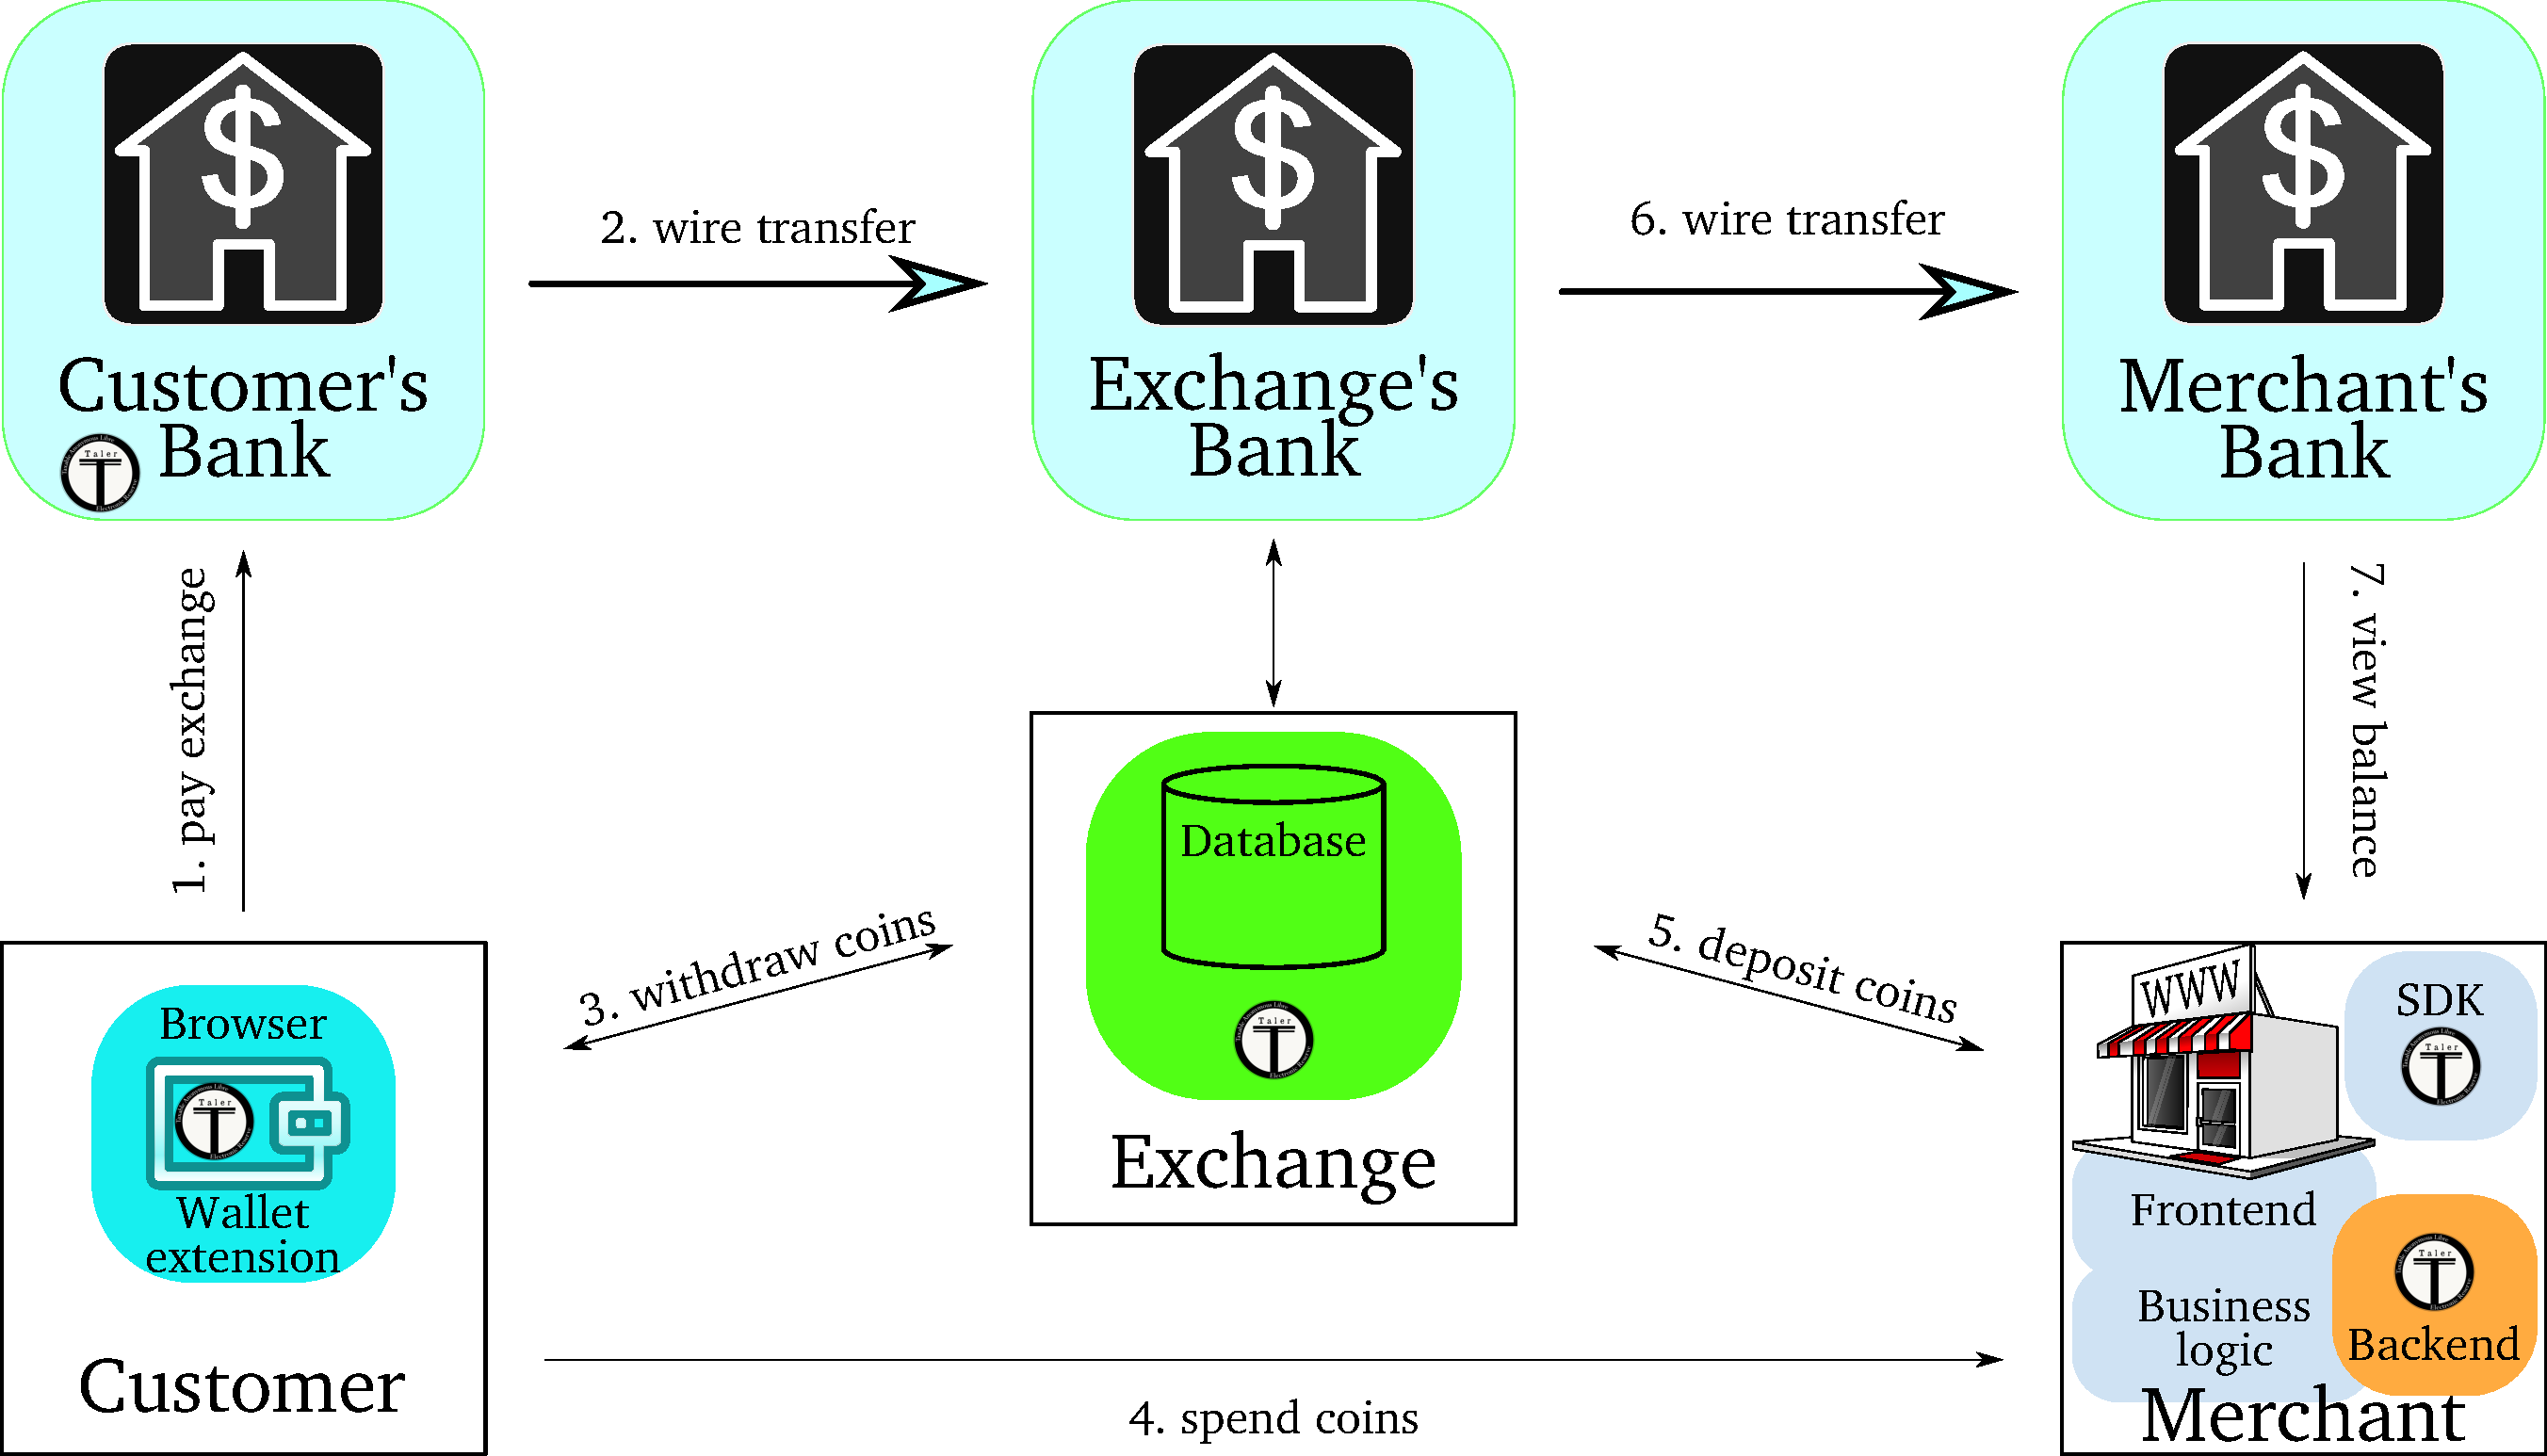
\includegraphics[width=\columnwidth]{taler-arch-full.pdf}
  \caption{The different components of the Taler system in the
    context of a banking system providing money creation,
    wire transfers and authentication. (Auditor omitted.)}
\end{figure}


\section{Experimental results}

%\begin{figure}[b!]
%    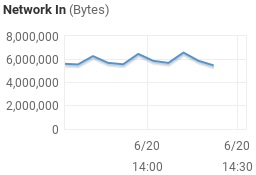
\includegraphics[width=\columnwidth]{bw_in.png}
%    \caption{Incoming traffic at the exchange, in bytes per 5 minutes.}
%    \label{fig:in}
%\end{figure}\hfill
%  \begin{figure}[b!]
%    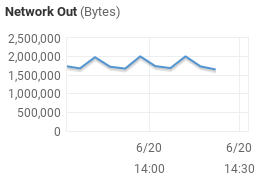
\includegraphics[width=\columnwidth]{bw_out.png}
%    \caption{Outgoing traffic from the exchange, in bytes per 5 minutes.}
%    \label{fig:out}
%  \end{figure}
%  \begin{figure}[b!]
%    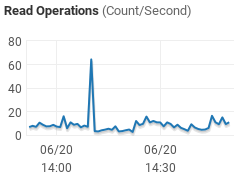
\includegraphics[width=\columnwidth]{db_read.png}
%    \caption{DB read operations per second.}
%    \label{fig:read}
%  \end{figure}
%  \begin{figure}[b!]
%    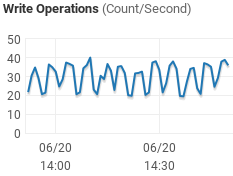
\includegraphics[width=\columnwidth]{db_write.png}
%    \caption{DB write operations per second.}
%    \label{fig:write}
%   \end{figure}
%  \begin{figure}[b!]
%    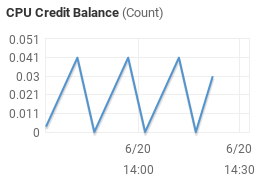
\includegraphics[width=\columnwidth]{cpu_balance.png}
%    \caption{CPU credit balance. Hitting a balance of 0 shows the CPU is
%       the limiting factor.}
%    \label{fig:cpu}
%  \end{figure}
%  \begin{figure}[b!]
%    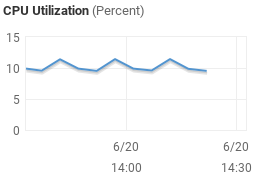
\includegraphics[width=\columnwidth]{cpu_usage.png}
%    \caption{CPU utilization. The t2.micro instance is allowed to use 10\% of
%       one CPU.}
%    \label{fig:usage}
%  \end{figure}
%  \caption{Selected EC2 performance monitors for the experiment in the EC2
%           (after several hours, once the system was ``warm'').}
%  \label{fig:ec2}
%\end{figure}

We ran the Taler exchange v0.0.2 on an Amazon EC2 t2.micro instance
(10\% of a Xeon E5-2676 at 2.4 GHz) based on Ubuntu 14.04.4 LTS, using
a db.t2.micro instance with Postgres 9.5 for the database.  We used
1024-bit RSA keys for blind signatures, Curve25519 for DH, EdDSA
for non-blind signatures and SHA-512 for hashing.  For the KDF and
FDH operations we used~\cite{rfc5869} with SHA-512 as XTR and SHA-256
for PRF as suggested in~\cite{rfc5869}.  Using 16
concurrent clients performing withdraw, deposit and refresh operations
we then pushed the t2.micro instance to the resource limit
%(Figure~\ref{fig:cpu})
from a network with $\approx$ 160 ms latency to
the EC2 instance.  At that point, the instance managed about 8 HTTP
requests per second, which roughly corresponds to one full business
transaction (as a full business transaction is expected to involve
withdrawing and depositing several coins).  The network traffic was
modest at approximately 50 kbit/sec from the exchange
%(Figure~\ref{fig:out})
and 160 kbit/sec to the exchange.
%(Figure~\ref{fig:in}).
At network latencies above 10 ms, the delay
for executing a transaction is dominated by the network latency, as
local processing virtually always takes less than 10 ms.

Database transactions are dominated by writes%
%(Figure~\ref{fig:read} vs.  Figure~\ref{fig:write})
, as Taler mostly needs to log
transactions and occasionally needs to read to guard against
double-spending.  Given a database capacity of 2 TB---which should
suffice for more than one year of full transaction logs---the
described setup has a hosting cost within EC2 of approximately USD 252
per month, or roughly 0.0001 USD per full business transaction.  This
compares favorably to the $\approx$ USD 10 per business transaction
for Bitcoin and the \EUR{0.35} plus 1.9\% charged by Paypal for
domestic transfers within Germany.

In the Amazon EC2 billing, the cost for the database (using SSD
storage) dominates the cost with more than USD 243 per month.  We note
that these numbers are approximate, as the frontend and backend in our
configuration uses systems from the AWS Free Usage Tier and is not
perfectly balanced in between frontend and backend.  Nevertheless,
these experimental results show that computing-related business costs
will only marginally contribute to the operational costs of the Taler
payment system.

Scalability of the design is also not a concern, as the exchange's
database can be easily shareded over the different public keys as
desired.  Similar to the RSCoin~\cite{danezis2016rscoin} design, this
ensures that conflicting transactions end up in the same shard,
enabling linear scalability of the database operations.  Similarly,
the cryptographic verification in the frontend can be distributed over
as many compute nodes as required.

\section{Discussion}

\subsection{Well-known attacks}

Taler's security is largely equivalent to that of Chaum's original
design without online checks or the cut-and-choose revelation of
double-spending customers for offline spending.
We specifically note that the digital equivalent of the ``Columbian
Black Market Exchange''~\cite{fatf1997} is a theoretical problem for
both Chaum and Taler, as individuals with a strong mutual trust
foundation can simply copy electronic coins and thereby establish a
limited form of black transfers.  However, unlike the situation with
physical checks with blank recipients in the Columbian black market,
the transitivity is limited as each participant can deposit the electronic
coins and thereby cheat any other participant, while in the Columbian
black market each participant only needs to trust the issuer of the
check and not also all previous owners of the physical check.

As with any unconditionally anonymous payment system, the ``Perfect
Crime'' attack~\cite{solms1992perfect} where blackmail is used to
force the exchange to issue anonymous coins also continues to apply in
principle.  However, as mentioned Taler does facilitate limits on
withdrawals, which we believe is a better trade-off than the
problematic escrow systems where the necessary intransparency
actually facilitates voluntary cooperation between the exchange and
criminals~\cite{sander1999escrow} and where the state could
deanonymize citizens.

\subsection{Offline Payments} \label{sec:offline}

Anonymous digital cash schemes since Chaum were frequently designed
to allow the merchant to be offline during the transaction,
by providing a means to deanonymize customers involved in
double-spending.  We consider this problematic as either the
exchange or the merchant still requires an out-of-band
means to recover funds from the customer, an expensive and
unreliable proposition.  Worse, there are unacceptable risks that
a customer may accidentally deanonymize herself, for example by
double-spending a coin after restoring from backup.

\subsection{Merchant Tax Audits}

For a tax audit on the merchant, the exchange includes the business
transaction-specific hash in the transfer of the traditional
currency.  A tax auditor can then request the merchant to reveal
(meaningful) details about the business transaction ($\mathcal{D}$,
$a$, $p$, $r$), including proof that applicable taxes were paid.

If a merchant is not able to provide theses values, they can be
subjected to financial penalties by the state in relation to the
amount transferred by the traditional currency transfer.

\subsection{Cryptographic proof vs. evidence}

In this paper we have use the term ``proof'' in many places as the
protocol provides cryptographic proofs of which parties behave
correctly or incorrectly. However, as~\cite{fc2014murdoch} point out,
in practice financial systems need to provide evidence that holds up
in courts.  Taler's implementation is designed to export evidence and
upholds the core principles described in~\cite{fc2014murdoch}.  In
particular, in providing the cryptographic proofs as evidence none of
the participants have to disclose their core secrets.

\subsection{Business concerns}

The Taler system implementation includes additional protocol elements
to address real-world concerns.  To begin with, the exchange
automatically transfers any funds that have been left for an extended
amount of time in a customer's reserve back to the customer's bank
account.  Furthermore, we allow the exchange to revoke denomination
keys, and wallets periodically check for such revocations.  If a
denomination key has been revoked, the wallets use the {\em payback}
protocol to deposit funds back to the customer's reserve, from where
they are either withdrawn with a new denomination key or sent back to
the customer's bank account.  Unlike ordinary deposits, the payback
protocol does not incur any transaction fees. The primary use of the
protocol is to limit the financial loss in cases where an audit
reveals that the exchange's private keys were compromised, and to
automatically pay back balances held in a customers' wallet if an
exchange ever goes out of business.


%\subsection{System Performance}
%
%We performed some initial performance measurements for the various
%operations on our exchange implementation.  The main conclusion was that
%the computational and bandwidth cost for transactions described in
%this paper is smaller than $10^{-2}$ cent/transaction, and thus
%dwarfed by the other business costs for the exchange.  However, this
%figure excludes the cost of currency transfers using traditional
%banking, which a exchange operator would ultimately have to interact with.
%Here, exchange operators should be able to reduce their expenses by
%aggregating multiple transfers to the same merchant.


\section{Conclusion}

We have presented an efficient electronic payment system that
simultaneously addresses the conflicting objectives created by the
citizen's need for privacy and the state's need for taxation.  The
coin refreshing protocol makes the design flexible and enables a
variety of payment methods.  The current balance and profits of the
exchange are also easily determined, thus audits can be used to ensure
that the exchange operates correctly.  The free software
implementation and open protocol may finally enable modern society to
upgrade to proper electronic wallets with efficient, secure and
privacy-preserving transactions.

% commented out for anonymized submission
\subsection*{Acknowledgements}

We thank people (anonymized).
%This work benefits from the financial support of the Brittany Region
%(ARED 9178) and a grant from the Renewable Freedom Foundation.
%We thank Tanja Lange, Dan Bernstein, Luis Ressel and Fabian Kirsch for feedback on an earlier
%version of this paper, Nicolas Fournier for implementing and running
%some performance benchmarks, and Richard Stallman, Hellekin Wolf,
%Jacob Appelbaum for productive discussions and support.
\newpage

\bibliographystyle{ACM-Reference-Format}
\bibliography{taler,rfc,rom}

%\end{document}

%\vfill
%\begin{center}
% \Large  Demonstration available at \url{https://demo.taler.net/}
%\end{center}
%\vfill

\newpage
\appendix

\section{Notation summary}

The paper uses the subscript $p$ to indicate public keys and $s$ to
indicate secret (private) keys.  For keys, we also use small letters
for scalars and capital letters for points on an elliptic curve.  The
capital letter without the subscript $p$ stands for the key pair.  The
superscript $(i)$ is used to indicate one of the elements of a vector
during the cut-and-choose protocol.  Bold-face is used to indicate a
vector over these elements.  A line above indicates a value computed
by the verifier during the cut-and-choose operation.  We use $f()$ to
indicate the application of a function $f$ to one or more arguments. Records of
data being persisted are represented in between $\langle\rangle$.

\begin{description}
  \item[$K_s$]{Denomination private (RSA) key of the exchange used for coin signing}
  \item[$K_p$]{Denomination public (RSA) key corresponding to $K_s$}
  \item[$K$]{Public-priate (RSA) denomination key pair $K := (K_s, K_p)$}
  \item[$\FDH_K$]{Full domain hash over the modulus of $K_p$}
  \item[$b$]{RSA blinding factor for RSA-style blind signatures}
  \item[$B_b()$]{RSA blinding over the argument using blinding factor $b$}
  \item[$U_b()$]{RSA unblinding of the argument using blinding factor $b$}
  \item[$S_K()$]{Chaum-style RSA signature, $S_K(C) = U_b(S_K(B_b(C)))$}
  \item[$w_s$]{Private key from customer for authentication}
  \item[$W_p$]{Public key corresponding to $w_s$}
  \item[$W$]{Public-private customer authentication key pair $W := (w_s, W_p)$}
  \item[$S_W()$]{Signature over the argument(s) involving key $W$}
  \item[$m_s$]{Private key from merchant for authentication}
  \item[$M_p$]{Public key corresponding to $m_s$}
  \item[$M$]{Public-private merchant authentication key pair $M := (m_s, M_p)$}
  \item[$S_M()$]{Signature over the argument(s) involving key $M$}
  \item[$G$]{Generator of the elliptic curve}
  \item[$c_s$]{Secret key corresponding to a coin, scalar on a curve}
  \item[$C_p$]{Public key corresponding to $c_s$, point on a curve}
  \item[$C$]{Public-private coin key pair $C := (c_s, C_p)$}
  \item[$S_{C}()$]{Signature over the argument(s) involving key $C$ (using EdDSA)}
  \item[$c_s'$]{Private key of a ``dirty'' coin (otherwise like $c_s$)}
  \item[$C_p'$]{Public key of a ``dirty'' coin (otherwise like $C_p$)}
  \item[$C'$]{Dirty coin (otherwise like $C$)}
  \item[$\widetilde{C}$]{Exchange signature $S_K(C_p)$ indicating validity of a fresh coin (with key $C$)}
  \item[$n$]{Number of exchanges accepted by a merchant}
  \item[$j$]{Index into a set of accepted exchanges, $i \in \{1,\ldots,n\}$}
  \item[$X_j$]{Public key of a exchange (not used to sign coins)}
  \item[$\vec{X}$]{Vector of $X_j$ signifying exchanges accepted by a merchant}
  \item[$a$]{Complete text of a contract between customer and merchant}
  \item[$f$]{Amount a customer agrees to pay to a merchant for a contract}
  \item[$m$]{Unique transaction identifier chosen by the merchant}
  \item[$H()$]{Hash function}
  \item[$p$]{Payment details of a merchant (i.e. wire transfer details for a bank transfer)}
  \item[$r$]{Random nonce}
  \item[${\mathcal A}$]{Complete contract signed by the merchant}
  \item[${\mathcal D}$]{Deposit permission, signing over a certain amount of coin to the merchant as payment and to signify acceptance of a particular contract}
  \item[$\kappa$]{Security parameter $\ge 3$}
  \item[$i$]{Index over cut-and-choose set, $i \in \{1,\ldots,\kappa\}$}
  \item[$\gamma$]{Selected index in cut-and-choose protocol, $\gamma \in \{1,\ldots,\kappa\}$}
  \item[$t^{(i)}_s$]{private transfer key, a scalar}
  \item[$T^{(i)}_p$]{public transfer key, point on a curve (same curve must be used for $C_p$)}
  \item[$T^{(i)}$]{public-private transfer key pair $T^{(i)} := (t^{(i)}_s,T^{(i)}_s)$}
  \item[$\vec{t}$]{Vector of $t^{(i)}_s$}
  \item[$c_s^{(i)}$]{Secret key corresponding to a fresh coin, scalar on a curve}
  \item[$C_p^{(i)}$]{Public key corresponding to $c_s^{(i)}$, point on a curve}
  \item[$C^{(i)}$]{Public-private coin key pair $C^{(i)} := (c_s^{(i)}, C_p^{(i)})$}
%  \item[$\vec{C}$]{Vector of $C^{(i)}$ (public and private keys)}
  \item[$b^{(i)}$]{Blinding factor for RSA-style blind signatures}
  \item[$\vec{b}$]{Vector of $b^{(i)}$}
  \item[$B^{(i)}$]{Blinding of $C_p^{(i)}$}
  \item[$\vec{B}$]{Vector of $B^{(i)}$}
  \item[$L^{(i)}$]{Link secret derived from ECDH operation via hashing}
%  \item[$E_{L^{(i)}}()$]{Symmetric encryption using key $L^{(i)}$}
%  \item[$E^{(i)}$]{$i$-th encryption of the private information $(c_s^{(i)}, b_i)$}
%  \item[$\vec{E}$]{Vector of $E^{(i)}$}
  \item[$\mathcal{R}$]{Tuple of revealed vectors in cut-and-choose protocol,
    where the vectors exclude the selected index $\gamma$}
  \item[$\overline{L^{(i)}}$]{Link secrets derived by the verifier from DH}
  \item[$\overline{B^{(i)}}$]{Blinded values derived by the verifier}
  \item[$\overline{T_p^{(i)}}$]{Public transfer keys derived by the verifier from revealed private keys}
  \item[$\overline{c_s^{(i)}}$]{Private keys obtained from decryption by the verifier}
  \item[$\overline{b_s^{(i)}}$]{Blinding factors obtained from decryption by the verifier}
  \item[$\overline{C^{(i)}_p}$]{Public coin keys computed from $\overline{c_s^{(i)}}$ by the verifier}
\end{description}

\end{document}






\section{Optional features}

In this appendix we detail various optional features that can
be added to the basic protocol to reduce transaction costs for
certain interactions.

However, we note that Taler's transaction costs are expected to be so
low that these features are likely not particularly useful in
practice: When we performed some initial performance measurements for
the various operations on our exchange implementation, the main conclusion
was that the computational and bandwidth cost for transactions
described in this paper is smaller than $10^{-3}$ cent/transaction,
and thus dwarfed by the other business costs for the exchange.  We note
that the $10^{-3}$ cent/transaction estimate excludes the cost of wire
transfers using traditional banking, which a exchange operator would
ultimately have to interact with.  Here, exchange operators should be able
to reduce their expenses by aggregating multiple transfers to the same
merchant.

As a result of the low cost of the interaction with the exchange in Taler
today, we expect that transactions with amounts below Taler's internal
transaction costs to be economically meaningless.  Nevertheless, we
document various ways how such transactions could be achieved within
Taler.



\subsection{Incremental spending}

For services that include pay-as-you-go billing, customers can over
time sign deposit permissions for an increasing fraction of the value
of a coin to be paid to a particular merchant.  As checking with the
exchange for each increment might be expensive, the coin's owner can
instead sign a {\em lock permission}, which allows the merchant to get
an exclusive right to redeem deposit permissions for the coin for a
limited duration.  The merchant uses the lock permission to determine
if the coin has already been spent and to ensure that it cannot be
spent by another merchant for the {\em duration} of the lock as
specified in the lock permission.  If the coin has insufficient funds
because too much has been spent or is
already locked, the exchange provides the owner's deposit or locking
request and signature to prove the attempted fraud by the customer.
Otherwise, the exchange locks the coin for the expected duration of the
transaction (and remembers the lock permission).  The merchant and the
customer can then finalize the business transaction, possibly
exchanging a series of incremental payment permissions for services.
Finally, the merchant then redeems the coin at the exchange before the
lock permission expires to ensure that no other merchant redeems the
coin first.

\begin{enumerate}
\item\label{offer2} The merchant sends an \emph{offer:}
  $\langle S_M(m, f), \vec{X} \rangle$ containing the price of the offer $f$,
  a transaction ID $m$ and the list of exchanges
   $\vec{X} = \langle X_1, \ldots, X_n \rangle$ accepted by the merchant,
   where each $X_j$ is an exchange's public key.
\item\label{lock2} The customer must possess or acquire a coin $\widetilde{C}$
  signed by a exchange that is accepted by the merchant,
   i.e.\ $K$ should be signed by some $X_j$ and has a value $\geq f$.

  Customer then generates a \emph{lock-permission}
  $\mathcal{L} := S_c(\widetilde{C}, t, m, f, M_p)$ where
  $t$ specifies the time until which the lock is valid and sends
  $\langle \mathcal{L}, X_j\rangle$ to the merchant,
  where $X_j$ is the exchange which signed $K$.
\item The merchant asks the exchange to apply the lock by sending $\langle
  \mathcal{L} \rangle$ to the exchange.
\item The exchange validates $\widetilde{C}$ and detects double spending
  in the form of existing \emph{deposit-permission} or
  lock-permission records for $\widetilde{C}$.  If such records exist
  and indicate that insufficient funds are left, the exchange sends those
  records to the merchant, who can then use the records to prove the double
  spending to the customer.

  If double spending is not found,
  the exchange persists $\langle \mathcal{L} \rangle$
  and notifies the merchant that locking was successful.
\item\label{contract2} The merchant creates a digitally signed contract
  \begin{equation*}
    \mathcal{A} := S_M(m, f, a, H(p, r))
  \end{equation*}
  where $a$ is data relevant to the contract
  indicating which services or goods the merchant will deliver to the customer, and $p$ is the
  merchant's payment information (e.g. his IBAN number) and $r$ is an random nonce.
  The merchant persists $\langle \mathcal{A} \rangle$ and sends it to the customer.
\item The customer creates a
  \emph{deposit-permission} $\mathcal{D} := S_c(\widetilde{C}, \widetilde{L}, f, m, M_p, H(a), H(p, r))$, persists
  $\langle \mathcal{A}, \mathcal{D} \rangle$ and sends $\mathcal{D}$ to the merchant.
\item\label{invoice_paid2} The merchant persists the received $\langle \mathcal{D} \rangle$.
\item The merchant gives $(\mathcal{D}, p, r)$ to the exchange, revealing his
  payment information.
\item The exchange verifies $(\mathcal{D}, p, r)$ for its validity and
  checks against double spending, while of
  course permitting the merchant to withdraw funds from the amount that
  had been locked for this merchant.
 \item If $\widetilde{C}$ is valid and no equivalent \emph{deposit-permission} for $\widetilde{C}$ and $\widetilde{L}$ exists, the
  exchange performs the following transaction:
  \begin{enumerate}
    \item $\langle \mathcal{D}, p, r \rangle$ is persisted.
    \item\label{transfer2} transfers an amount of $f$ to the merchant's bank account
      given in $p$.  The subject line of the transaction to $p$ must contain
      $H(\mathcal{D})$.
  \end{enumerate}
  Finally, the exchange sends a confirmation to the merchant.
 \item If the deposit record $\langle \mathcal{D}, p, r \rangle$ already exists,
  the exchange sends the confirmation to the merchant,
  but does not transfer money to $p$ again.
\end{enumerate}

To facilitate incremental spending of a coin $C$ in a single transaction, the
merchant makes an offer in Step~\ref{offer2} with a maximum amount $f_{max}$ he
is willing to charge in this transaction from the coin $C$.  After obtaining the
lock on $C$ for $f_{max}$, the merchant makes a contract in Step~\ref{contract2}
with an amount $f \leq f_{max}$.  The protocol follows with the following steps
repeated after Step~\ref{invoice_paid2} whenever the merchant wants to charge an
incremental amount up to $f_{max}$:

\begin{enumerate}
  \setcounter{enumi}{4}
\item The merchant generates a new contract $ \mathcal{A}' := S_M(m, f', a', H(p,
  r)) $ after obtaining the deposit-permission for a previous contract.  Here
  $f'$ is the accumulated sum the merchant is charging the customer, of which
  the merchant has received a deposit-permission for $f$ from the previous
  contract \textit{i.e.}~$f <f' \leq f_{max}$.  Similarly $a'$ is the new
  contract data appended to older contract data $a$.
  The merchant persists $\langle \mathcal{A}' \rangle$ and sends it to the customer.
\item Customer persists $\langle \mathcal{A}' \rangle$, creates
  $\mathcal{D}' := S_c(\widetilde{C}, \mathcal{L}, f', m, M_p, H(a'), H(p, r))$, persists
  $\langle \mathcal{D'} \rangle$ and sends it to the merchant.
\item The merchant persists the received $\langle \mathcal{D'} \rangle$ and
  deletes the older $\mathcal{D}$.
\end{enumerate}

%Figure~\ref{fig:spending_protocol_interactions} summarizes the interactions of the
%coin spending protocol.

For transactions with multiple coins, the steps of the protocol are
executed in parallel for each coin.  During the time a coin is locked,
the locked fraction may not be spent at a different merchant or via a
deposit permission that does not contain $\mathcal{L}$.  The exchange will
release the locks when they expire or are used in a deposit operation.
Thus the coins can be used with other merchants once their locks
expire, even if the original merchant never executed any deposit for
the coin.  However, doing so may link the new transaction to older
transaction.

Similarly, if a transaction is aborted after Step 2, subsequent
transactions with the same coin can be linked to the coin, but not
directly to the coin's owner.  The same applies to partially spent
coins.  Thus, to unlink subsequent transactions from a coin, the
customer has to execute the coin refreshing protocol with the exchange.

%\begin{figure}[h]
%\centering
%\begin{tikzpicture}
%
%\tikzstyle{def} = [node distance= 1em, inner sep=.5em, outer sep=.3em];
%\node (origin) at (0,0) {};
%\node (offer) [def,below=of origin]{make offer (merchant $\rightarrow$ customer)};
%\node (A) [def,below=of offer]{permit lock (customer $\rightarrow$ merchant)};
%\node (B) [def,below=of A]{apply lock (merchant $\rightarrow$ exchange)};
%\node (C) [def,below=of B]{confirm (or refuse) lock (exchange $\rightarrow$ merchant)};
%\node (D) [def,below=of C]{sign contract (merchant $\rightarrow$ customer)};
%\node (E) [def,below=of D]{permit deposit (customer $\rightarrow$ merchant)};
%\node (F) [def,below=of E]{make deposit (merchant $\rightarrow$ exchange)};
%\node (G) [def,below=of F]{transfer confirmation (exchange $\rightarrow$ merchant)};
%
%\tikzstyle{C} = [color=black, line width=1pt]
%\draw [->,C](offer) -- (A);
%\draw [->,C](A) -- (B);
%\draw [->,C](B) -- (C);
%\draw [->,C](C) -- (D);
%\draw [->,C](D) -- (E);
%\draw [->,C](E) -- (F);
%\draw [->,C](F) -- (G);
%
%\draw [->,C, bend right, shorten <=2mm] (E.east)
%      to[out=-135,in=-45,distance=3.8cm] node[left] {aggregate} (D.east);
%\end{tikzpicture}
%\caption{Interactions between a customer, merchant and exchange in the coin spending
%  protocol}
%\label{fig:spending_protocol_interactions}
%\end{figure}


\subsection{Probabilistic donations}

Similar to Peppercoin, Taler supports probabilistic {\em micro}donations of coins to
support cost-effective transactions for small amounts.  We consider
amounts to be ``micro'' if the value of the transaction is close or
even below the business cost of an individual transaction to the exchange.

To support microdonations, an ordinary transaction is performed based
on the result of a biased coin flip with a probability related to the
desired transaction amount in relation to the value of the coin.  More
specifically, a microdonation of value $\epsilon$ is upgraded to a
macropayment of value $m$ with a probability of $\frac{\epsilon}{m}$.
Here, $m$ is chosen such that the business transaction cost at the
exchange is small in relation to $m$.  The exchange is only involved in the
tiny fraction of transactions that are upgraded.  On average both
customers and merchants end up paying (or receiving) the expected
amount $\epsilon$ per microdonation.

Unlike Peppercoin, in Taler either the merchant wins and the customer
looses the coin, or the merchant looses and the customer keeps the
coin.  Thus, there is no opportunity for the merchant and the customer
to conspire against the exchange.  To determine if the coin is to be
transferred, merchant and customer execute a secure coin flipping
protocol~\cite{blum1981}.  The commit values are included in the
business contract and are revealed after the contract has been signed
using the private key of the coin.  If the coin flip is decided in
favor of the merchant, the merchant can redeem the coin at the exchange.

One issue in this protocol is that the customer may use a worthless
coin by offering a coin that has already been spent.  This kind of
fraud would only be detected if the customer actually lost the coin
flip, and at this point the merchant might not be able to recover from
the loss.  A fraudulent anonymous customer may run the protocol using
already spent coins until the coin flip is in his favor.

As with incremental spending, lock permissions could be used to ensure
that the customer cannot defraud the merchant by offering a coin that
has already been spent.  However, as this means involving the exchange
even if the merchant looses the coin flip, such a scheme is unsuitable
for microdonations as the transaction costs from involving the exchange
might be disproportionate to the value of the transaction, and thus
with locking the probabilistic scheme has no advantage over simply
using fractional payments.

Hence, Taler uses probabilistic transactions {\em without} online
double-spending detection.  This enables the customer to defraud the
merchant by paying with a coin that was already spent.  However, as,
by definition, such microdonations are for tiny amounts, the incentive
for customers to pursue this kind of fraud is limited.  Still, to
clarify that the customer must be honest, we prefer the term
micro{\em donations} over micro{\em payments} for this scheme.


The following steps are executed for microdonations with upgrade probability $p$:
\begin{enumerate}
  \item The merchant sends an offer to the customer.
  \item The customer sends a commitment $H(r_c)$ to a random
    value $r_c \in [0,2^R)$, where $R$ is a system parameter.
  \item The merchant sends random $r_m \in [0,2^R)$ to the customer.
    \item The customer computes $p' := (|r_c - r_m|) / (2^R)$.
    If $p' < p$, the customer sends a coin with deposit-permission to the merchant.
    Otherwise, the customer sends $r_c$ to the merchant.
  \item The merchant deposits the coin, or checks if $r_c$ is consistent
    with $H(r_c)$.
\end{enumerate}

Evidently the customer can ``cheat'' by aborting the transaction in
Step 3 of the microdonation protocol if the outcome is unfavorable ---
and repeat until he wins.  This is why Taler is suitable for
microdonations --- where the customer voluntarily contributes ---
and not for micropayments.

Naturally, if the donations requested are small, the incentive to
cheat for minimal gain should be quite low.  Payment software could
embrace this fact by providing an appeal to conscience in form of an
option labeled ``I am unethical and want to cheat'', which executes
the dishonest version of the payment protocol.

If an organization detects that it cannot support itself with
microdonations, it can always choose to switch to the macropayment
system with slightly higher transaction costs to remain in business.

\newpage



Taler was designed for use in a modern social-liberal society and
provides a payment system with the following key properties:

\begin{description}
  \item[Customer Anonymity]
    It is impossible for exchanges, merchants and even a global active
    adversary, to trace the spending behavior of a customer.
    As a strong form of customer anonymity, it is also infeasible to
    link a set of transactions to the same (anonymous) customer.
    %, even when taking aborted transactions into account.

    There is, however, a risk of metadata leakage if a customer
    acquires coins matching exactly the price quoted by a merchant, or
    if a customer uses coins issued by multiple exchanges for the same
    transaction.  Hence, our implementation does not allow this.

  \item[Taxability]
    In many current legal systems, it is the responsibility of the merchant
    to deduct sales taxes from purchases made by customers, or for workers
    to pay income taxes for payments received for work.
    Taler ensures that merchants are easily identifiable and that
    an audit trail is generated, so that the state can ensure that its
    taxation regime is obeyed.
  \item[Verifiability]
    Taler minimizes the trust necessary between
    participants.  In particular, digital signatures are retained
    whenever they would play a role in resolving disputes.
    Additionally, customers cannot defraud anyone, and
    merchants can only defraud their customers by not
    delivering on the agreed contract.  Neither merchants nor customers
    are able to commit fraud against the exchange.
    Only the exchange needs be tightly audited and regulated.
  \item[No speculation] % It's actually "Speculation not required"
    The digital coins are denominated in existing currencies,
    such as EUR or USD.  This avoids exposing citizens to unnecessary risks
    from currency fluctuations.
  \item[Low resource consumption]
    The design minimizes the operating costs and environmental impact of
    the payment system.  It uses few public key operations per
    transaction and entirely avoids proof-of-work computations.
    The payment system handles both small and large payments in
    an efficient and reliable manner.
\end{description}
